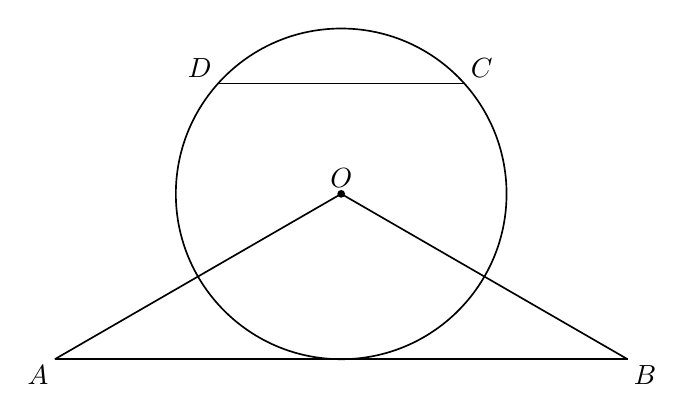
\begin{tikzpicture}[x=1cm,y=1cm,line width=.6pt,font=\normalsize]
\coordinate (O) at (0,0);
\coordinate (A) at (-3.637307,-2.1);
\coordinate (B) at (3.637307,-2.1);
\coordinate (D) at (-1.565248,1.4);
\coordinate (C) at (1.565248,1.4);
\draw (O) circle[radius=2.1cm];
\draw (O)--(A);
\draw (O)--(B);
\draw (A)--(B);
\draw (D)--(C);
\node[above=2pt,inner sep=0pt] at (O) {$O$};
\node[below left=2pt,inner sep=0pt] at (A) {$A$};
\node[below right=2pt,inner sep=0pt] at (B) {$B$};
\node[above left=2pt,inner sep=0pt] at (D) {$D$};
\node[above right=2pt,inner sep=0pt] at (C) {$C$};

% Explicit named circle-center points, painted after all region fills.
\fill (O) circle[radius=1.4pt];
\end{tikzpicture}
